\documentclass[12pt]{article}

\usepackage{sbc-template}

\usepackage{graphicx,url}

\usepackage[brazil]{babel}  

\usepackage[utf8]{inputenc}  
     
\title{Avaliação de Algoritmos de Previsão de Desvio\\por meio do Simulador gem5}

\author{Elio Bolognese Neto\inst{1}}

\address{Departamento de Informática -- Universidade Estadual de Maringá (UEM)\\
87.020-900 -- Maringá -- PR -- Brasil
\email{eliobzgt@gmail.com}
}

\begin{document} 

\maketitle

\section{Introdução}

De acordo com \cite{yeh1991two}, o \textit{pipeline} é a melhor forma de tornar um processador único mais eficaz. No entanto, os desvios afetam no desempenho do processador pois precisam esperar que determinadas instruções sejam concluídas para que o destino possa ser buscado, gerando assim as “bolhas” no \textit{pipeline}. A perda de desempenho torna-se considerável quando são necessários vários ciclos para resolver o desvio.

Existem algumas formas de diminuir essa perda de desempenho. Entre elas, tem-se a previsão de desvio, que, como o nome diz, tenta prever se o desvio será tomado ou não. Isto é feito por meio de regras pré-determinadas, podendo ser estática (é única durante toda a execução) ou dinâmica (se adapta conforme a execução). Este segundo geralmente é mais eficiente, pois tenta aprender com os erros já cometidos.

São várias as abordagens para algoritmos de previsão de desvio dinâmica. Por isso, neste trabalho serão observados alguns desses algoritmos, executando-os em alguns programas por meio do simulador gem5 no modo de operação \textit{System-call Emulation}, para então compará-los em quesito de eficiência e visualizar o desempenho deles em tipos distintos de programas.

\section{Simulador gem5}
	
"A infraestrutura do simulador gem5 é uma combinação dos melhores aspectos dos simuladores M5 e GEMS. O M5 fornece um framework de simulação altamente configurável, múltiplas ISAs, e diversos modelos de CPU. O GEMS complementa esses recursos com um detalhado e flexível sistema de memória, incluindo suporte para múltiplos protocolos de coerência de cache e modelos de interconexão"\cite{binkert2011gem5}.

As ISAs (Instruction set architecture) que são suportadas nessa ferramenta são ALPHA, ARM, MIPS, Power, SPARC e x86. Os modelos de CPU presentes no gem5 são \textit{AtomicSimple}, \textit{TimingSimple}, \textit{InOrder} e O3. Em questão de memória, os sistemas que podem ser utilizados são \textit{Classic} e \textit{Ruby}.

O gem5 possui dois modos de operação, o \textit{System-call Emulation} (SE), que emula a maioria das instruções em nível de sistema sem a necessidade de um SO (Sistema Operacional), e o \textit{Full-System} (FS), que modela em nível de usuário e de kernel um sistema completo, fazendo necessário a instalação de um SO.

\section{Algoritmos de previsão de desvio}

Para evitar que o pipeline tenha que ser limpo quando um salto precisa ser tomado e já tenha entrado outras instruções, gastando tempo desnecessário, ou então bloquear a entrada de novas instruções até que seja decidido na fase de execução se o salto será ou não tomado, gerando bolhas no pipeline, os microprocessadores atuais utilizam algoritmos de previsão de desvio, que prevêem logo na fase de decodificação se o salto será tomado. “As previsões são baseadas em um cache chamado \textit{Branch Target Buffer} (BTB), que armazena o histórico de desvios dos saltos e faz predições de acordo com esse histórico”\cite{colin2000worst}.

Por existirem várias abordagens para fazer as previsões, também existem vários algoritmos de previsão de desvio. Neste trabalho, foram selecionados quatro algoritmos diferentes: LocalBP, TournamentBP, BiModeBP e LTAGE.

\subsection{LocalBP}

Esse algoritmo, segundo \cite{mcfarling1993combining}, utiliza duas tabelas de vetores para tomar a decisão de se o salto será ou não tomado. A primeira tabela guarda o histórico dos saltos mais recentes. Por não armazenar qual o salto que é previsto, ele considera todos os saltos como iguais, assim, perdendo desempenho por errar várias vezes. A segunda tabela é composta por contadores de dois bits indexados ao histórico da outra tabela. Ela é atualizada sempre que um salto é executado, incrementando se o salto é tomado, ou decrementando caso não seja tomado. Sendo assim, quanto mais esse algoritmo acerta, mais tempo o contador permanecerá prevendo a mesma ação. 

Os contadores dessa tabela são saturados, assim, por serem de dois bits, não podem ficar menor que zero ou maior que três. Portanto, duas falhas seguidas na previsão fazem com que o algoritmo troque o tipo de previsão que estava fazendo.

\subsection{TournamentBP}

"O TournamentBP utiliza dois ou mais preditores, geralmente um baseado em informações globais e um baseado em informações locais, combinando-os com um seletor, para realizar a previsão"\cite{hennessy2011computer}. Os preditores usam um contador de 2 bits saturado por salto para escolher entre os diferentes preditores com base em qual foi mais eficaz nas previsões mais recentes. 

\subsection{BiModeBP}

Esse algoritmo "divide as tabelas de previsão em duas metades e, determinando dinamicamente o modo atual do programa, seleciona a metade apropriada da tabela para previsão"\cite{lee1997bi}. Esta abordagem é utilizada pois não impacta no desempenho do processador e melhora a precisão da previsão.

\subsection{LTAGE}

De acordo com \cite{seznec2007256},	o TAGE é um preditor dependente de várias tabelas de previsão indexadas por funções independentes dos saltos. Ele se utiliza de componentes de outros tipos de preditores para fazer as melhores previsões possíveis com relação tanto aos saltos mais recentes quanto aos antigos também. O LTAGE é um tipo de preditor TAGE, na qual possui 13 componentes unidos por um preditor de loop de 256 entradas.

\section{Avaliação}

Os experimentos foram realizados numa máquina virtual de arquitetura Intel$^{®}$ Xeon$^{®}$ E5-2699
v3 com 8 núcleos e 15GB de memória RAM. O sistema operacional instalado é o Ubuntu 16.04.4 LTS x64, com kernel 4.13.0-1011. 

Foi utilizado o simulador gem5 no modo SE (\textit{System-call Emulation}) com a arquitetura x86 e o tipo binário \textit{fast}.

Os programas executados foram: mvt, retirado do PolyBench/C 4.1, jpeg\_c, retirado do cBench\_V1.1, trie, queens e perlin, retirados do LLVM test suit.

\begin{figure}[!htbp]
	
	\centering
	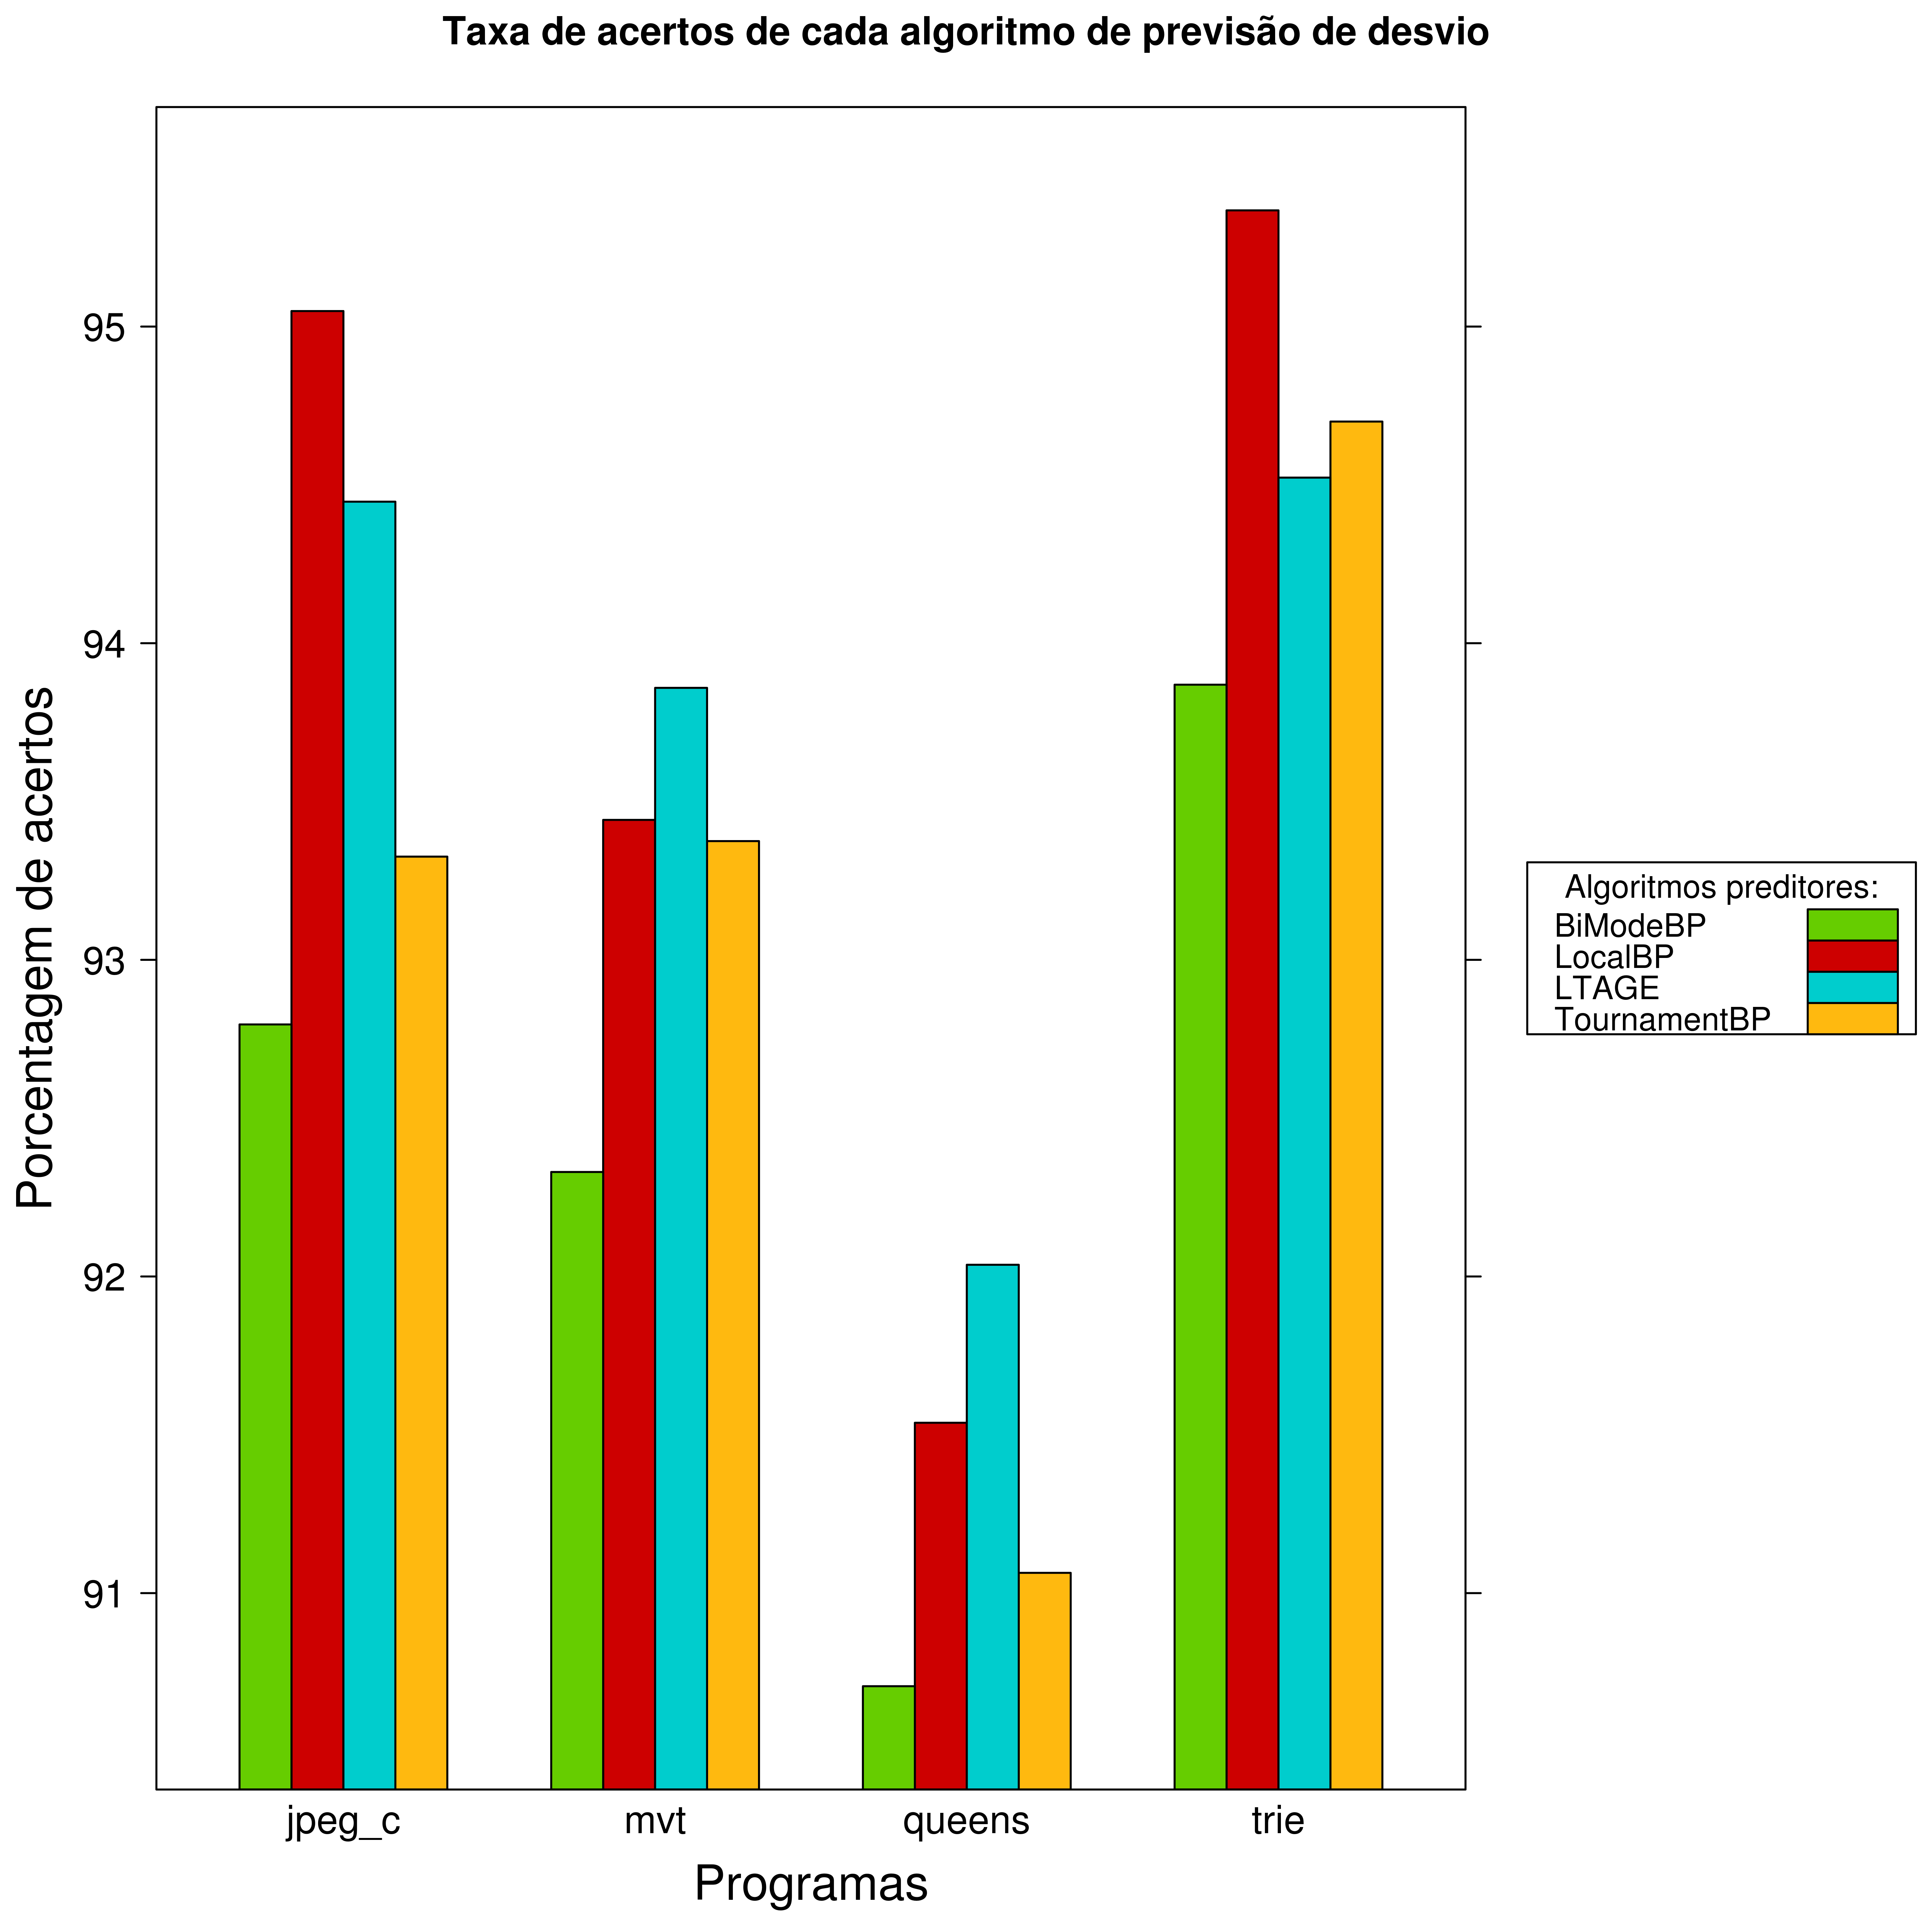
\includegraphics[scale=0.25]{Taxa_Acertos.png}
	\caption{Taxa de acertos de previsão de saltos condicionais de cada algoritmo em cada programa}
	\label{figura1}
    
\end{figure}

\begin{figure}[!htbp]
	
	\centering
	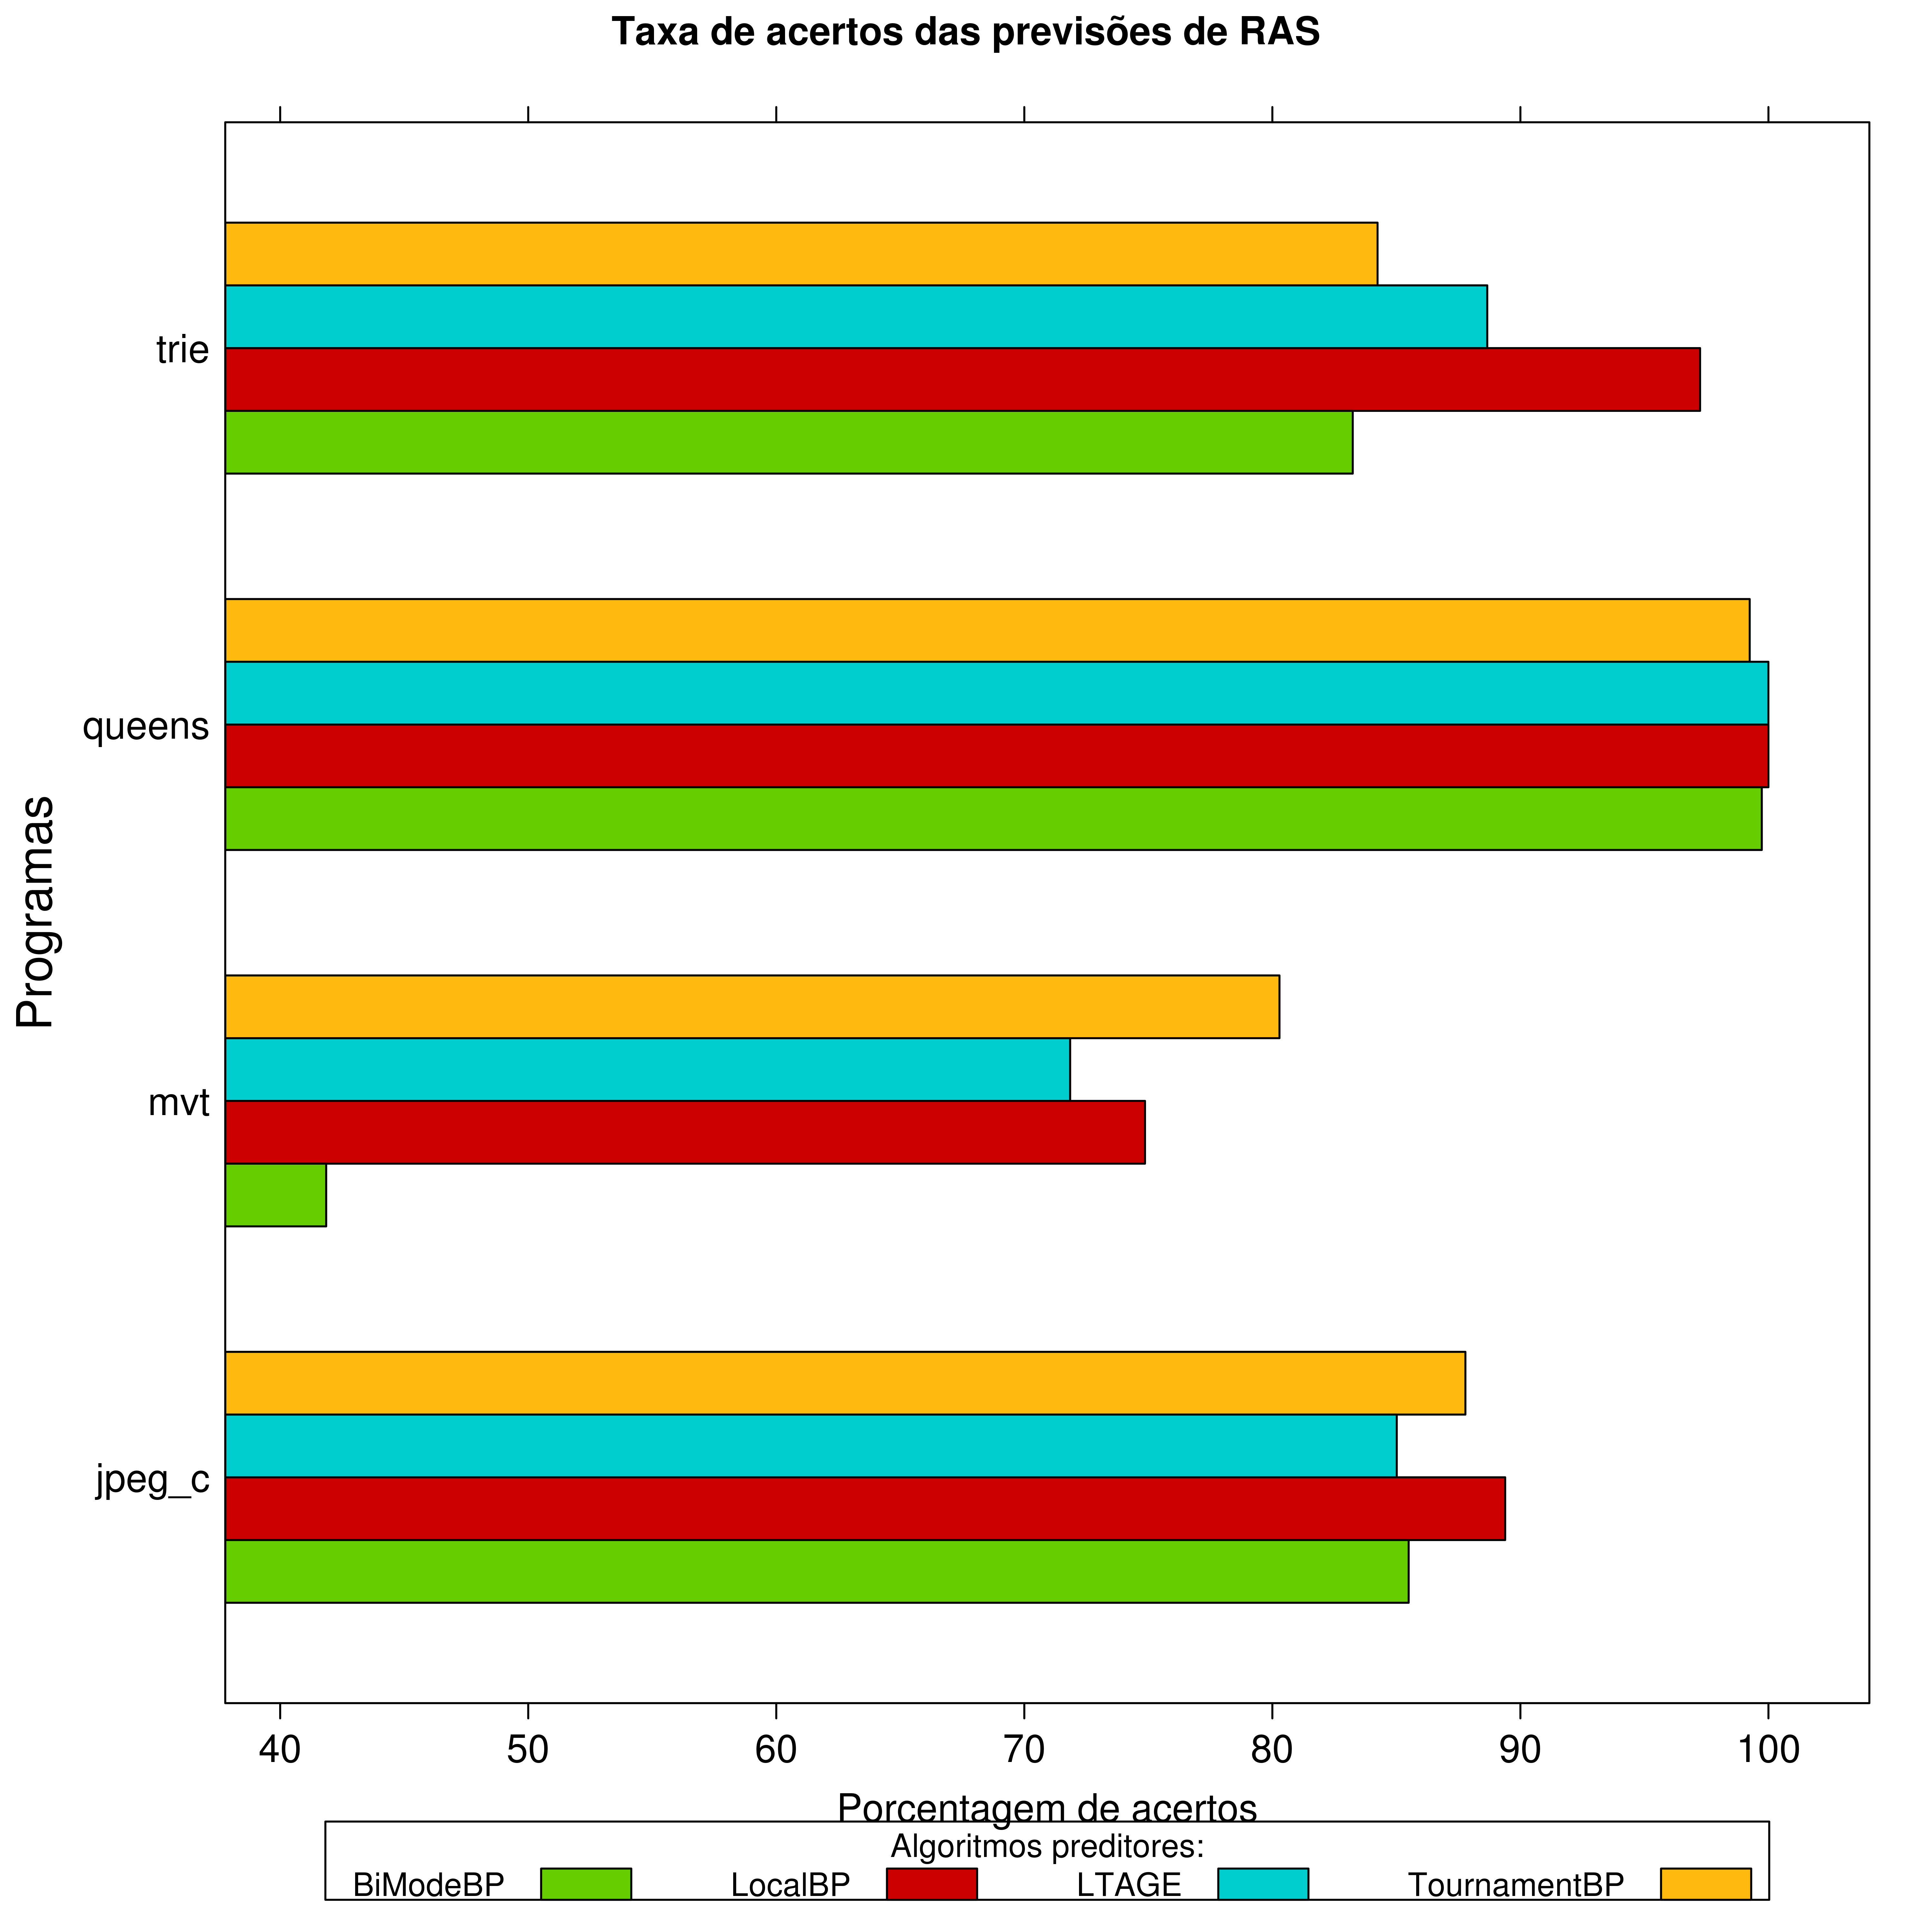
\includegraphics[scale=0.25]{Taxa_Acertos_RAS.png}
	\caption{Taxa de acertos de previsão de saltos de retorno de funções de cada algoritmo em cada programa}
	\label{figura2}
    
\end{figure}

\subsection{mvt}

Esse programa faz o produto vetorial de uma matriz e transposta. É possível observar pela Figura \ref{figura1} que os algoritmos de previsão de desvio selecionados tem uma perda de desempenho quando trabalho com algoritmos que utilizam matrizes, ficando numa faixa de 6 a 8\% de erros. A perda de desempenho é maior quando se trata de RAS (\textit{Return Address Stack}), como mostra na Figura \ref{figura2}, na qual houve caso em que a taxa de erro foi maior que  de acerto. 

\subsection{jpeg\_c}

Este programa utiliza uma biblioteca de rotinas para converter um arquivo JPEG para algum outro formato famoso de imagens. Pela Figura \ref{figura1}, nota-se que, por usarem abordagens diferentes, nem todos os algoritmos de previsão de desvio trabalham bem com conversões de arquivos.

\begin{figure}[!htbp]
	
	\centering
	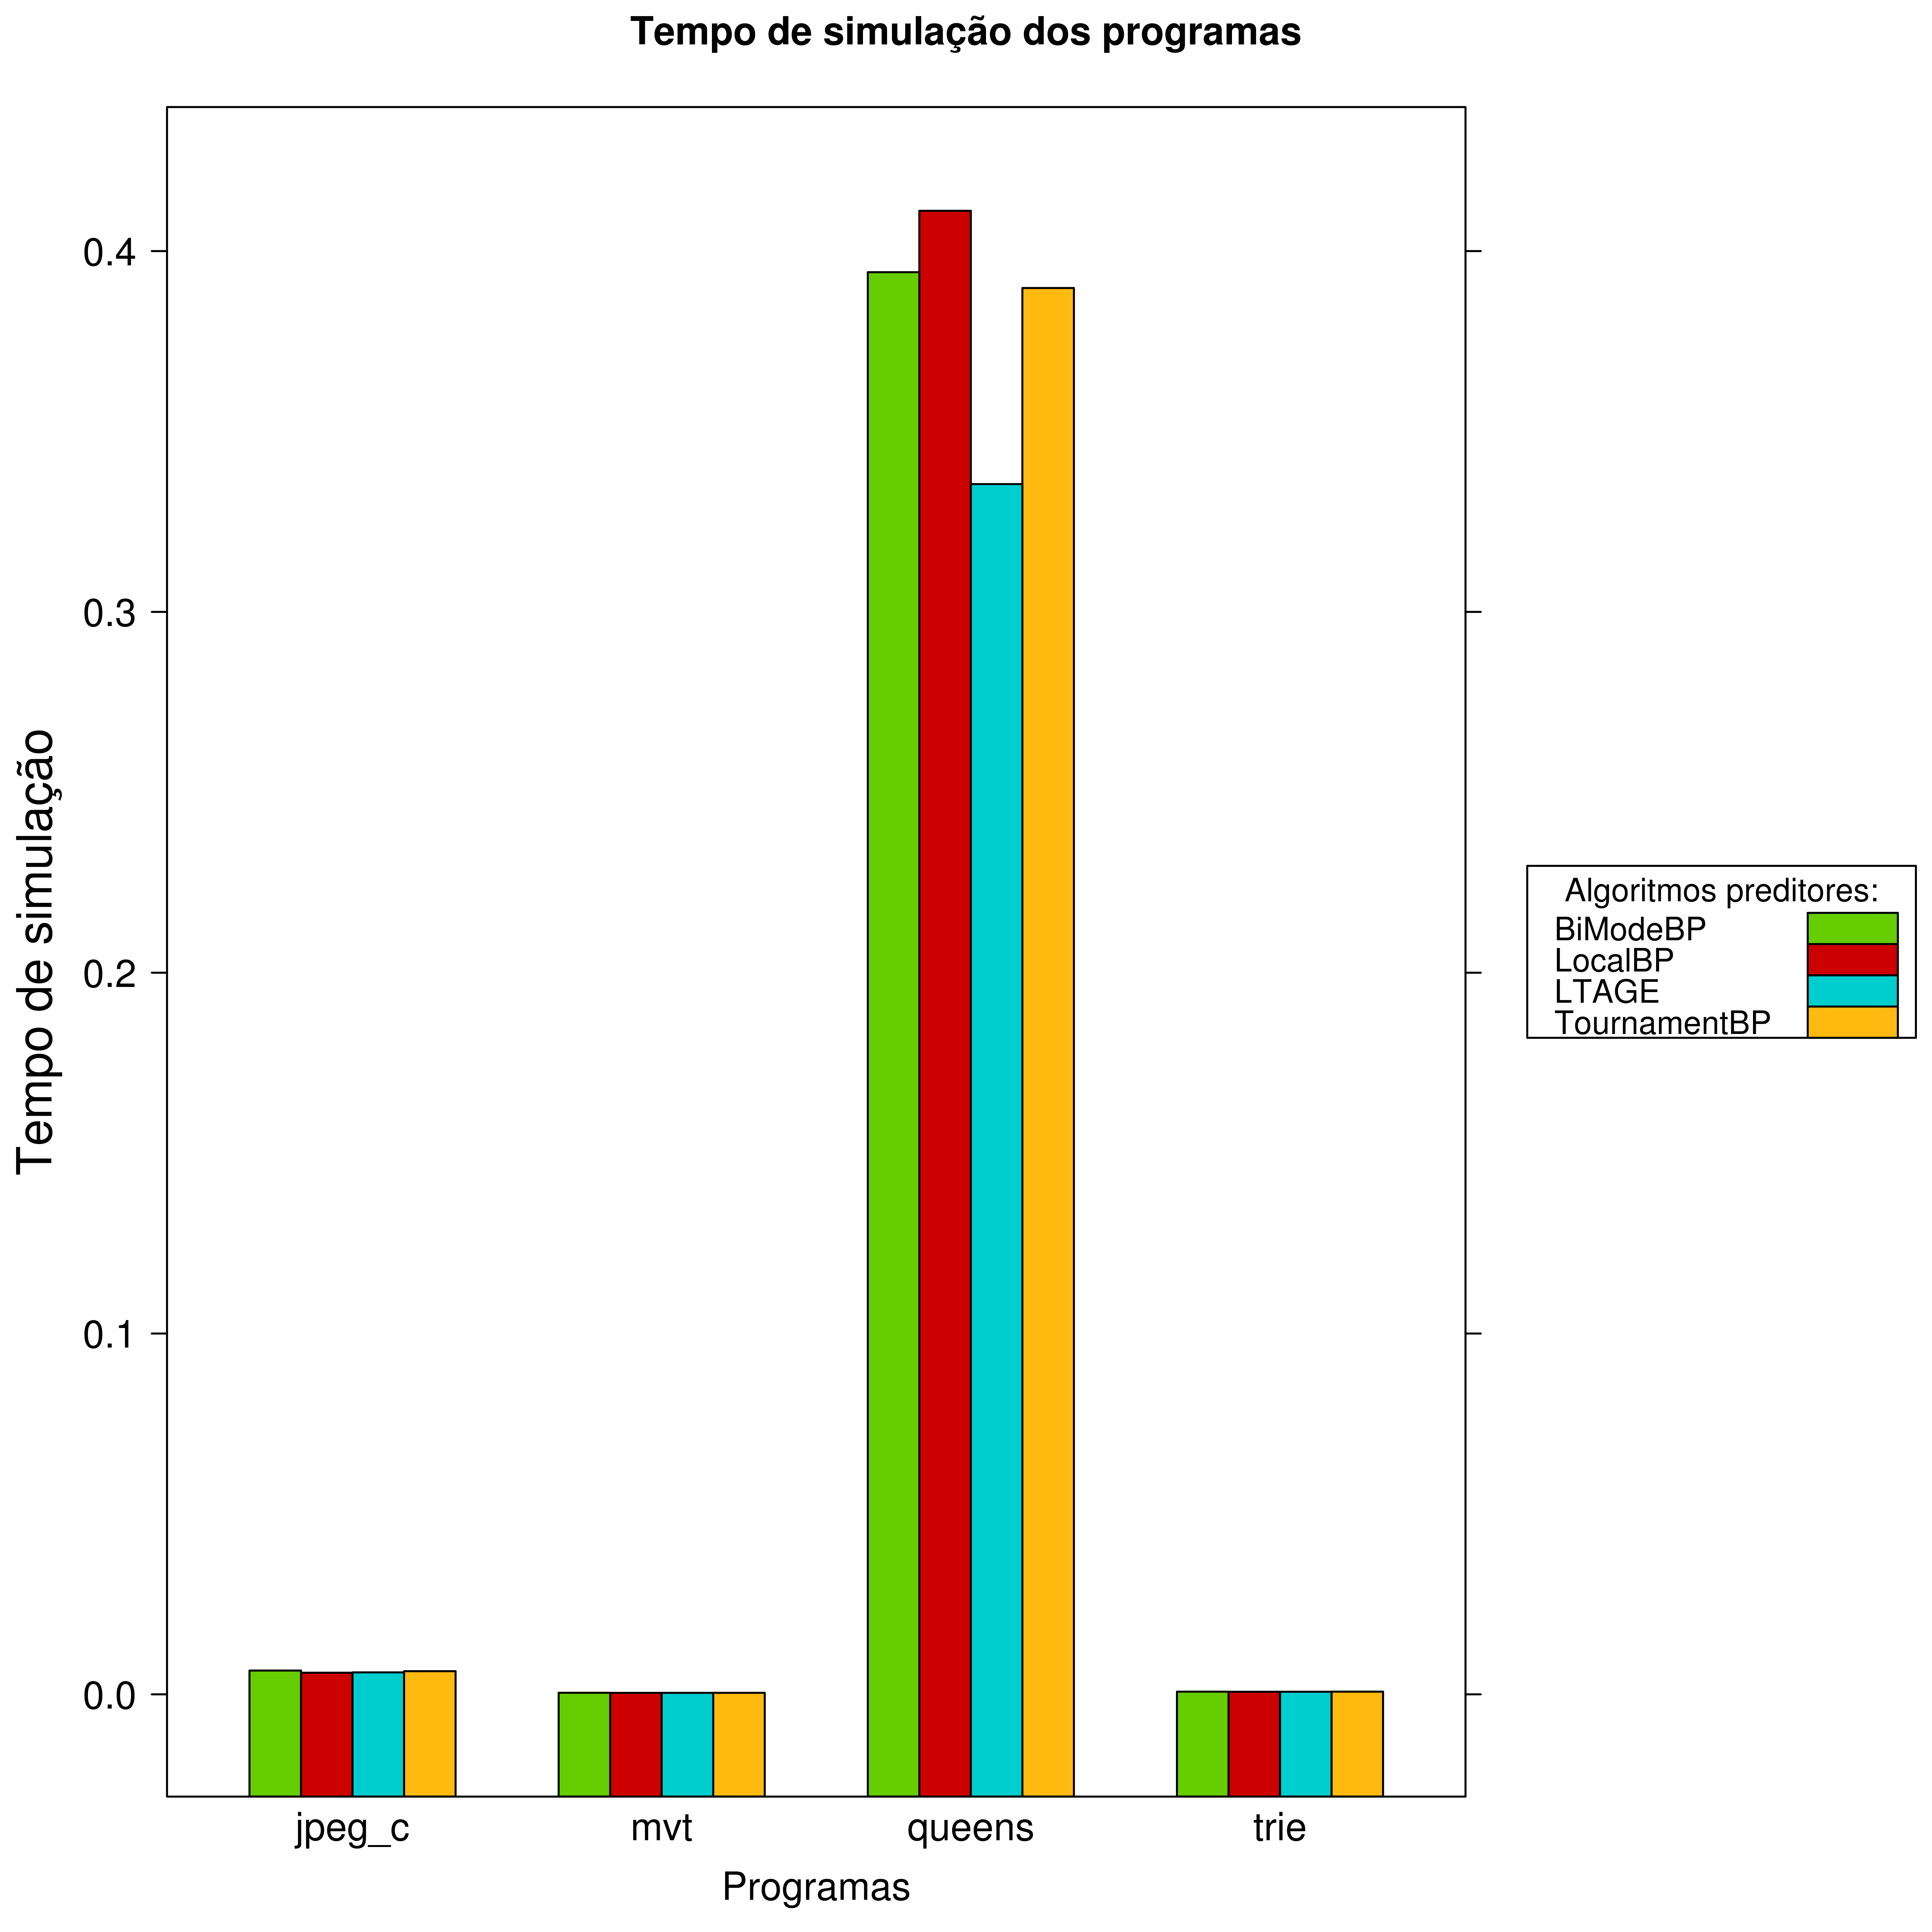
\includegraphics[scale=0.25]{Tempo_Execucao.png}
	\caption{Tempo de simulação utilizado pelos algoritmos em cada programa}
	\label{figura3}
	
\end{figure}

\begin{figure}[!htbp]
	
	\centering
	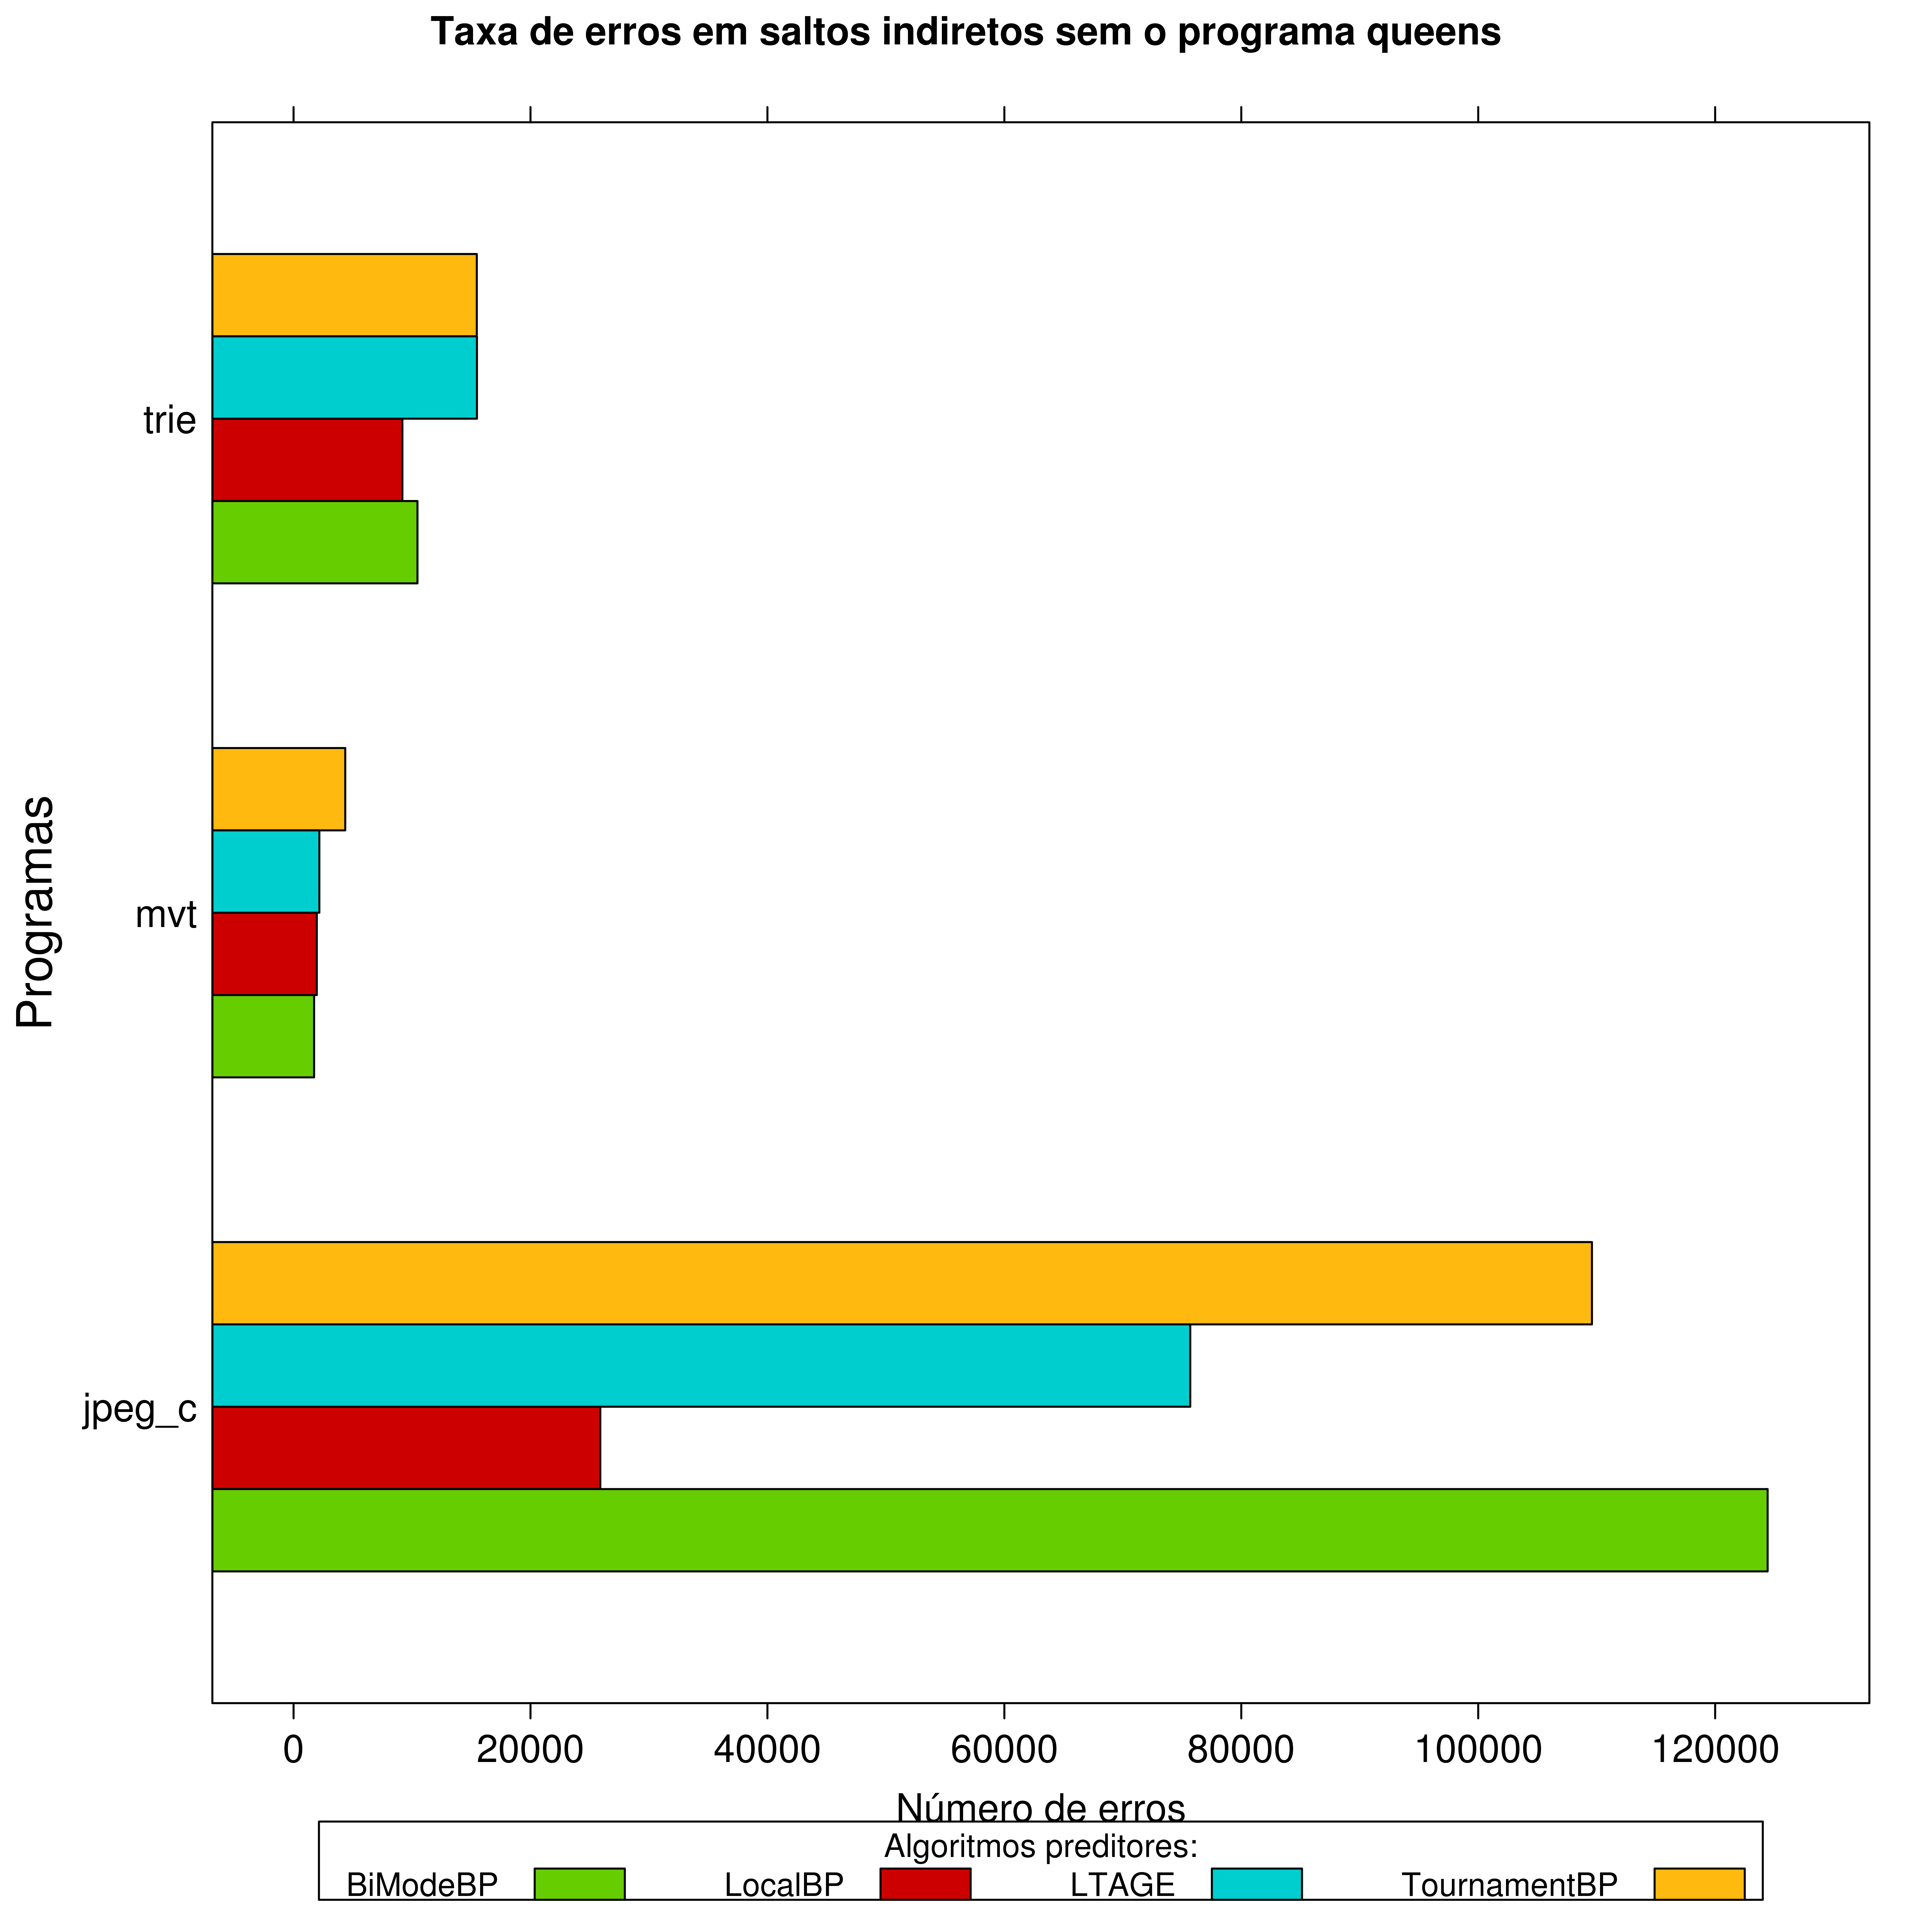
\includegraphics[scale=0.25]{Taxa_Miss_No_Queens.png}
	\caption{Taxa de acertos de previsão de saltos indiretos de cada algoritmo nos programas mais rápidos}
	\label{figura4}
	
\end{figure}

\subsection{trie}

Esse programa recebe um arquivo e tenta corrigir algum comportamento indevido que tiver nele. Na Figura \ref{figura3} e na Figura \ref{figura4} vemos que, embora o tempo de execução seja muito pequeno, a quantidade de previsões indiretas incorretas é considerável. No entanto, a Figura \ref{figura1} mostra que os algoritmos conseguem prever bem os saltos quando há entrada de strings.

\begin{figure}[!htbp]
	
	\centering
	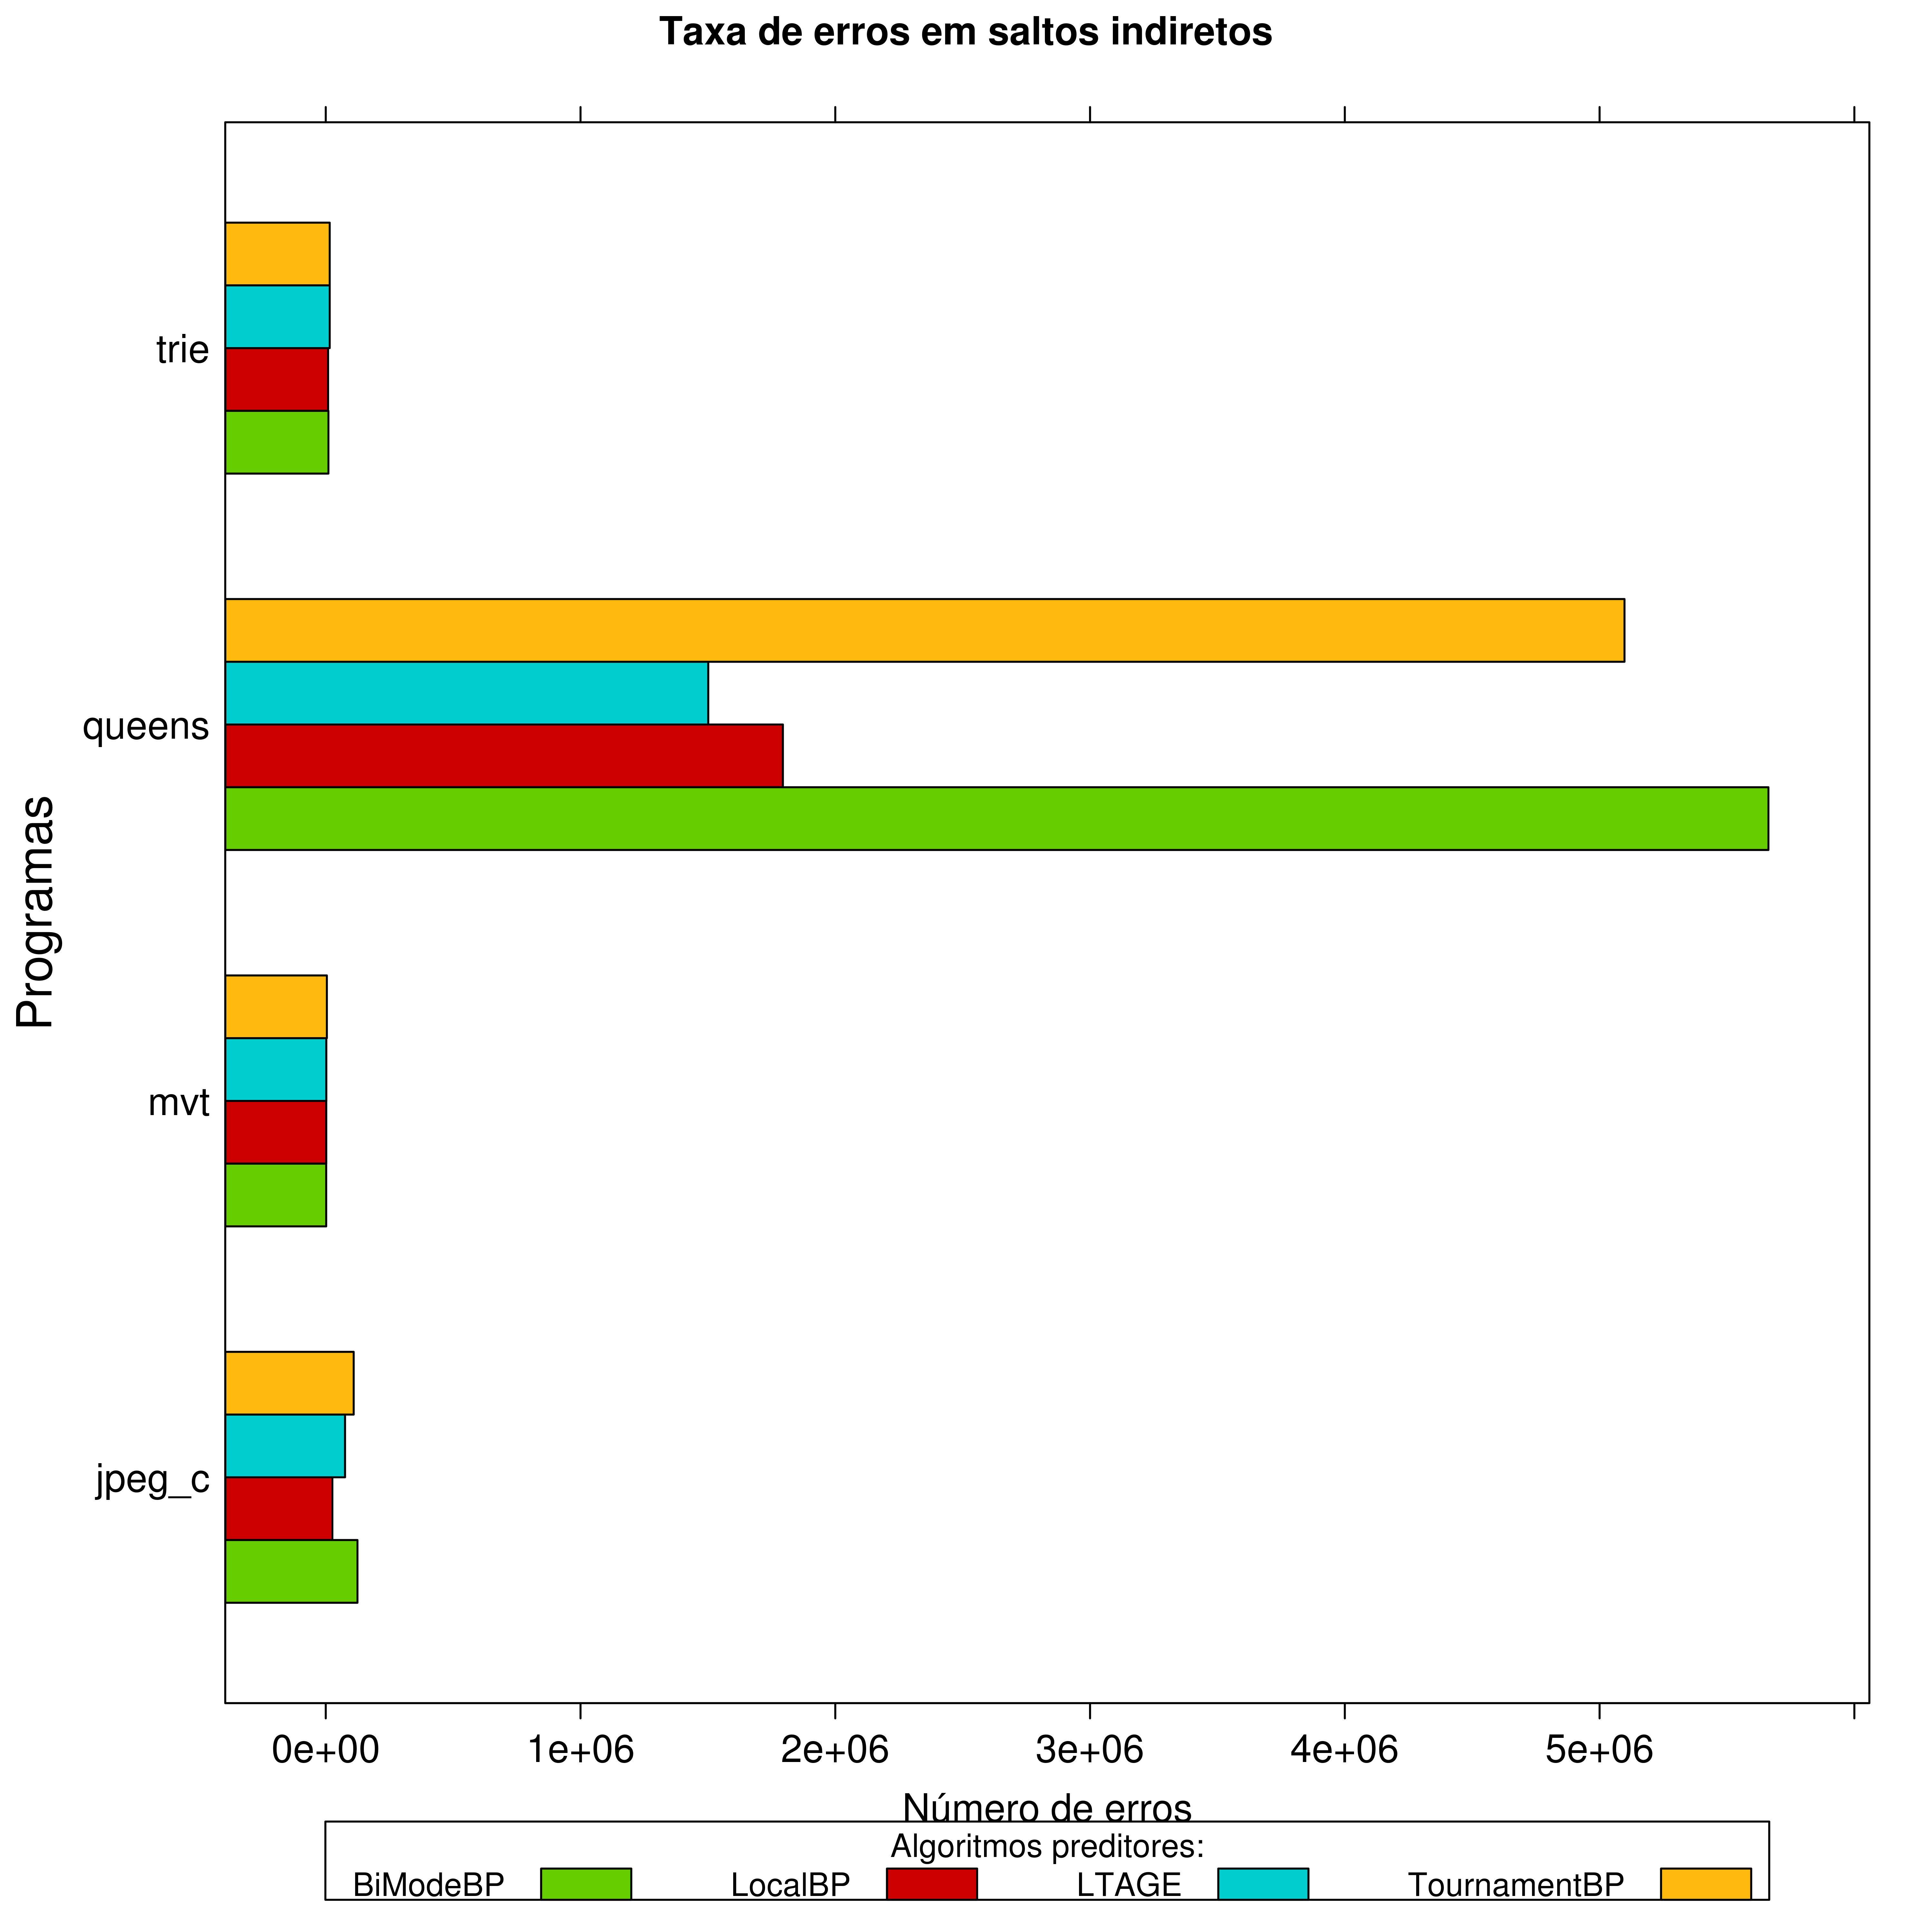
\includegraphics[scale=0.25]{Taxa_Miss_Indirect.png}
	\caption{Taxa de acertos de previsão de saltos indiretos de cada algoritmo em cada programa}
	\label{figura5}
	
\end{figure}

\subsection{queens}

Este programa encontra todas as maneiras possíveis que N rainhas podem ser colocadas em um tabuleiro de xadrez NxN de modo que as rainhas não possam capturar umas às outras. Dos programas que conseguimos analisar, vemos na Figura \ref{figura3} que esse foi o que levou o maior tempo para concluir sua execução. Entretanto, se observarmos a Figura \ref{figura5}, vemos que isso não influência totalmente na quantidade de erros de previsão indireta, mas sim a abordagem usada nesses algoritmos. Por outro lado, podemos concordar com o que foi dito anteriormente sobre o desempenho em matrizes olhando a Figura \ref{figura1}.

\subsection{perlin}

Esse programa produz texturas com aparência natural em superfícies geradas por computação gráfica para efeitos visuais de filmes. Embora tenha ficado executando durante quase uma semana, a execução não foi concluída, logo, não foi possível analisar o desempenho dos algoritmos nesse programa. 

\section{Conclusão}

Os algoritmos de previsão de desvio são importantes por aumentar o desempenho dos processadores pois tentam manter o pipeline cheio com informções corretas o maior tempo possível. Por ser dinâmico, ele aprende durante a execução, isso que dizer que existe várias abordagens diferentes para fazer esse algoritmo funcionar corretamente. Assim, existem vários preditores de desvio, cada um com suas vantagens e desvantagens.

Nesse trabalho foram testados os algoritmos de previsão de desvio LocalBP, TournamentBP, BiModeBP e LTAGE, nos programas mvt, jpeg\_c, trie, queens e perlin que realizam tarefas variadas. Eles foram executados no simulador gem5, que consegue simular quase que uma arquitetura completa. Ao término das execuções, foram avaliados alguns dos dados gerados de cada algoritmo.

Com isso, pudemos concluir que, mesmo alguns sendo mais antigos, os algoritmos testados conseguem melhorar o desempenho do processador prevendo em mais de 90\% das vezes o resultado dos saltos. Além disso, também foi observado que não existe um algoritmo preditor que é superior a todos os outros, mas sim aqueles que se sobressaem mais do que outros em determinadas instâncias.

\bibliographystyle{sbc}

\bibliography{sbc-template}

\end{document}